We introduce a stereo-vision based system that enables automatic event detection based on detection and tracking of vehicles in scenarios that usually would be highly problematic for monocular detectors. The purpose is to provides insight into patterns and behaviors of drivers during near-crashes and crashes. The proposed system will be limited to only handling a handful of events, which especially benefit from the extra dimension gained with stereo-vision. The considered events are illustrated in Figure \ref{fig:introduction:semantics}. 
%\vspace*{-3mm}
\begin{figure}[H]
  \centering
  \begin{tabular}{lr}
    \subfloat[\tiny{Average number of cars in front of ego-vehicle.}]{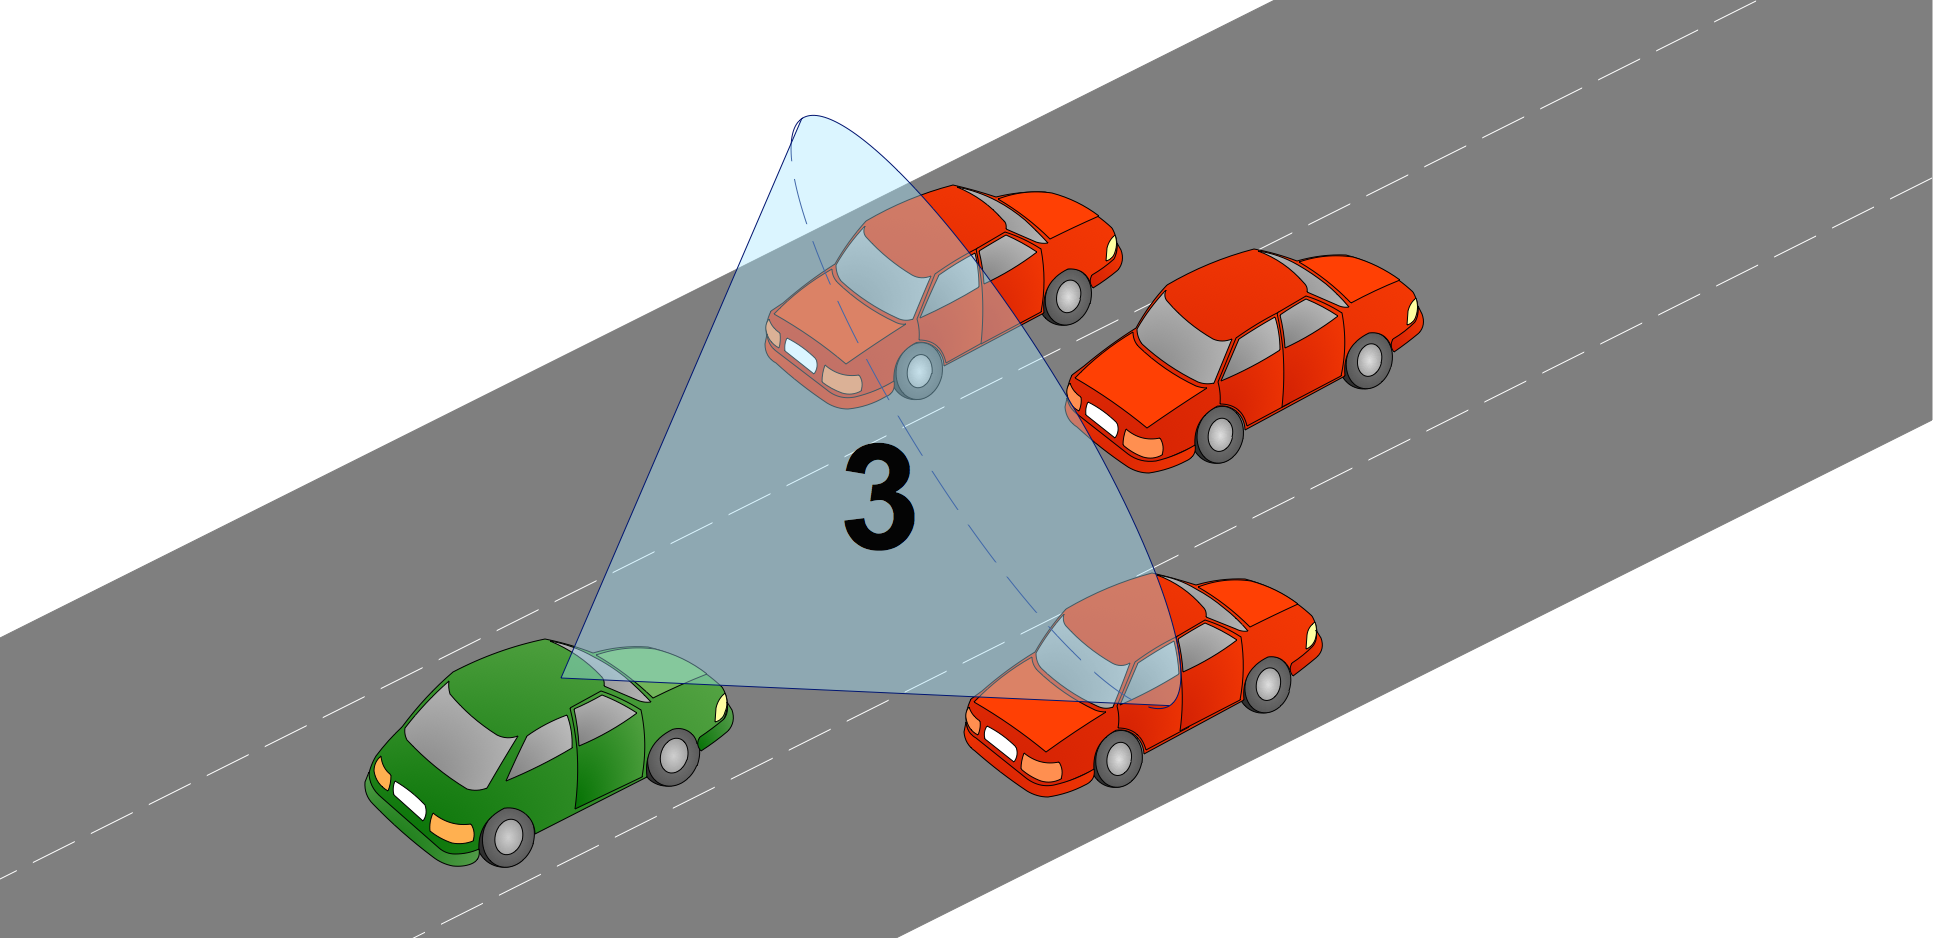
\includegraphics[width=0.45\textwidth]{text/figures/numOfObjects.png} \label{fig:introduction:semantics:a}} &
    \subfloat[\tiny{Distance to rear-end of vehicle directly in front.}]{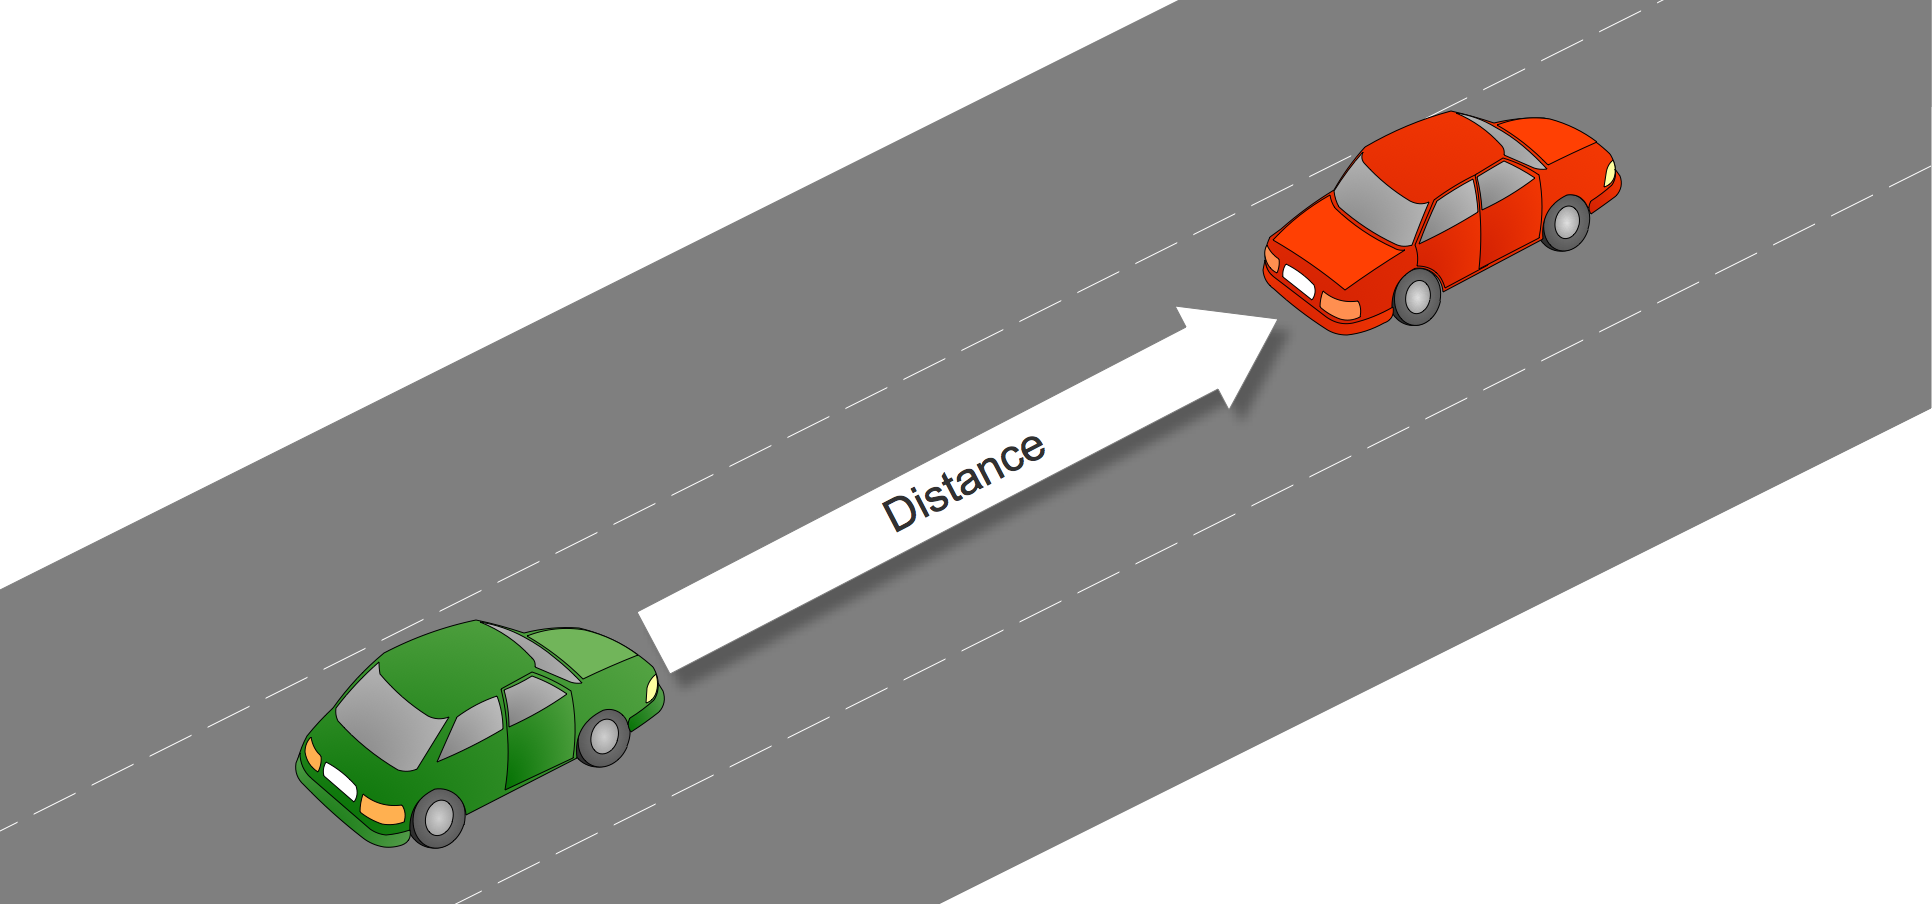
\includegraphics[width=0.45\textwidth]{text/figures/avgDistanceSameLane.png} \label{fig:introduction:semantics:b}} \\
    
    \subfloat[\tiny{Other vehicle entering intersection - turning onto opposite direction.}]{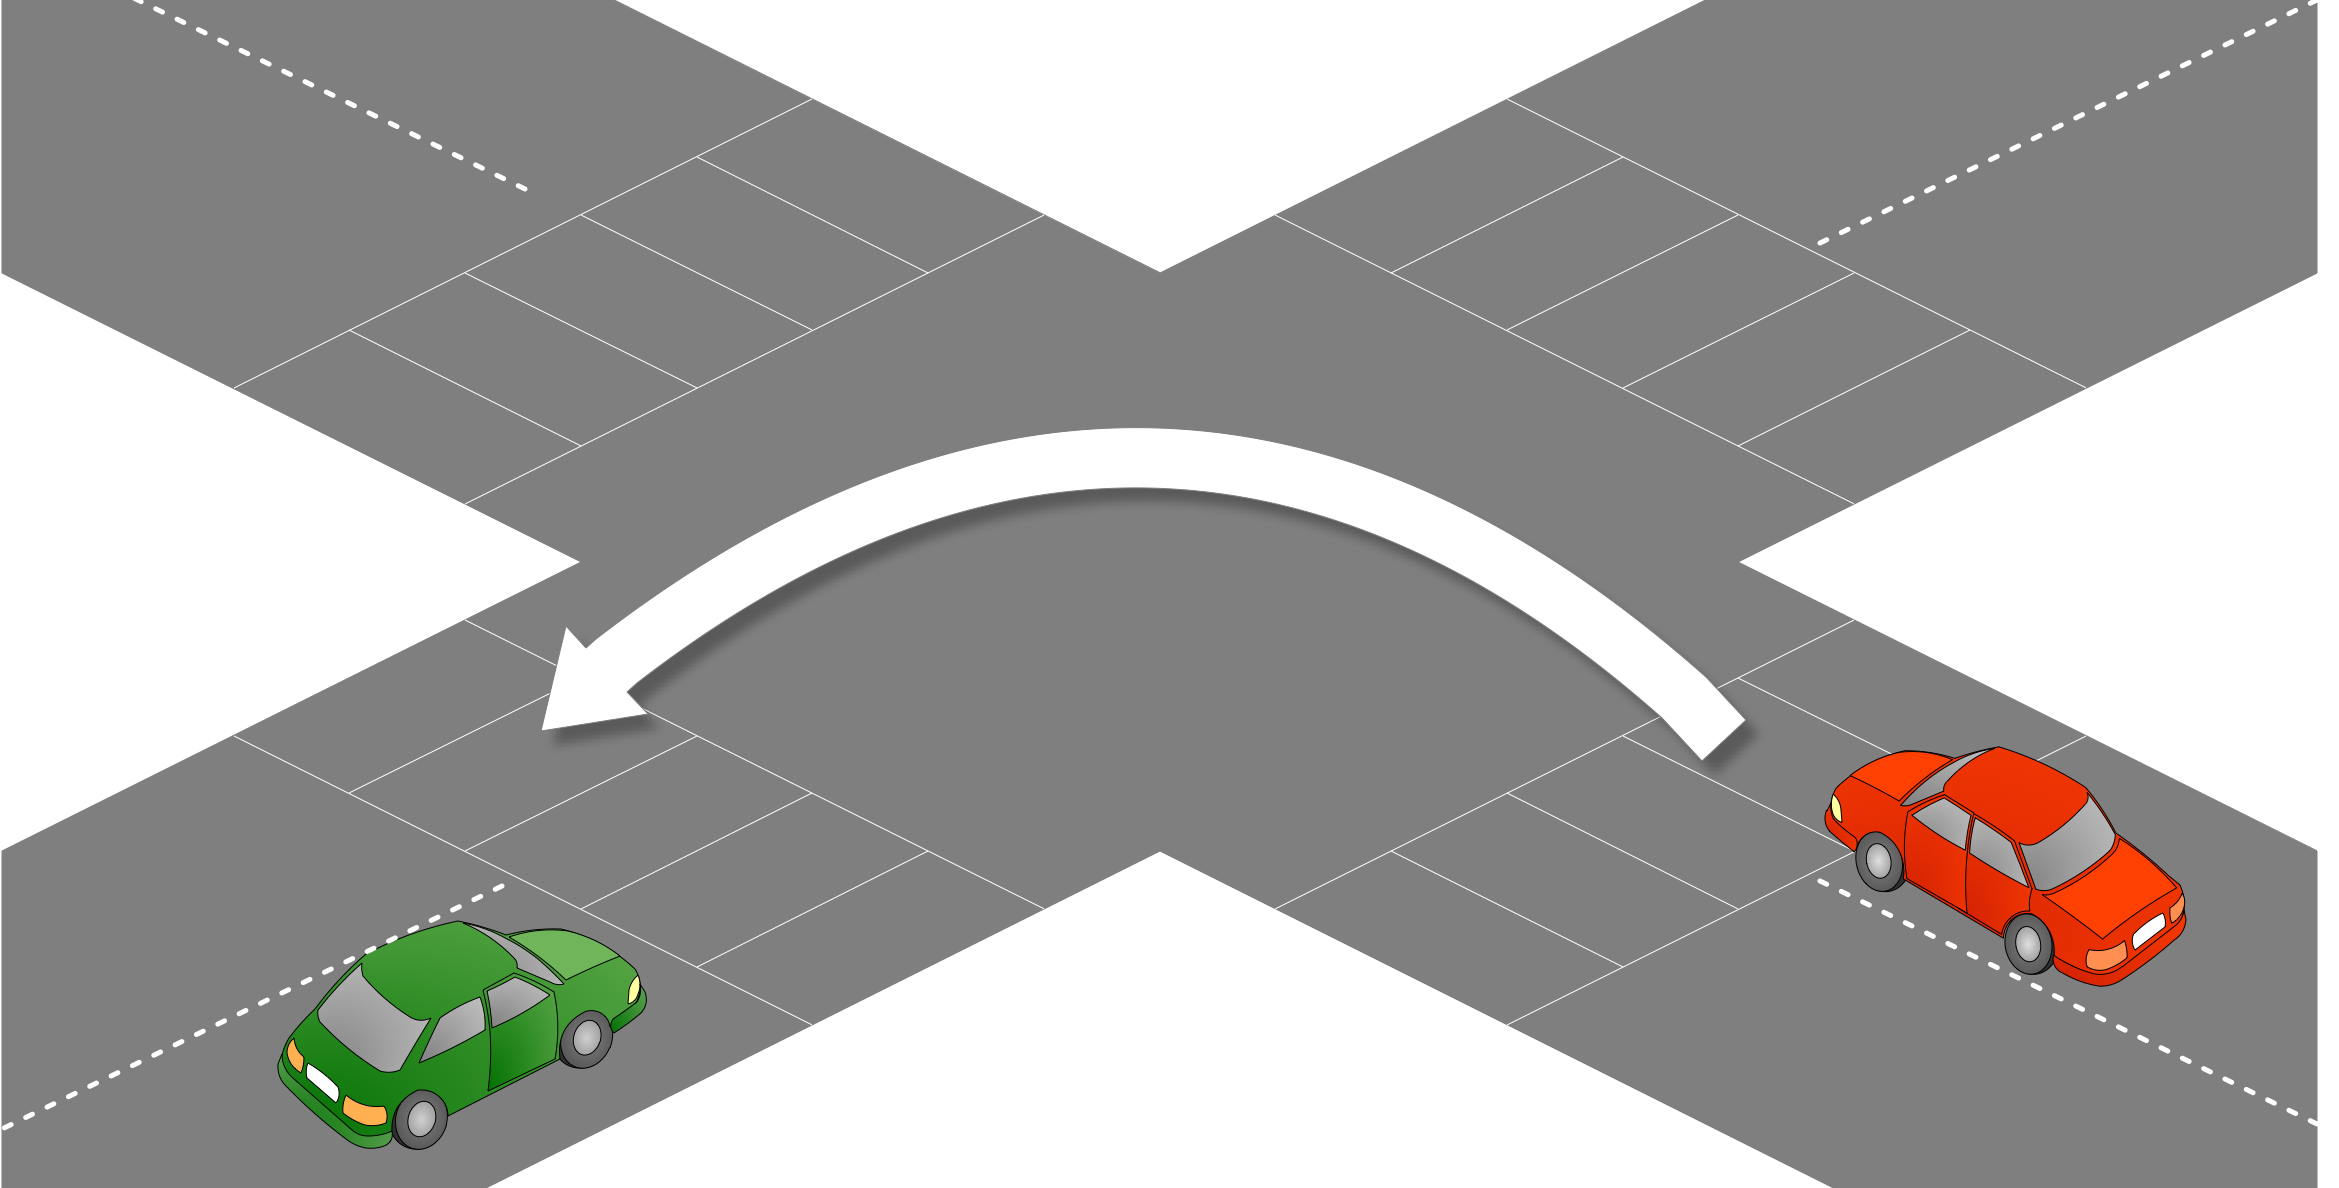
\includegraphics[width=0.45\textwidth]{text/figures/turningO.png} \label{fig:introduction:semantics:c}} &
    \subfloat[\tiny{Other vehicle entering intersection - left turn across path.}]{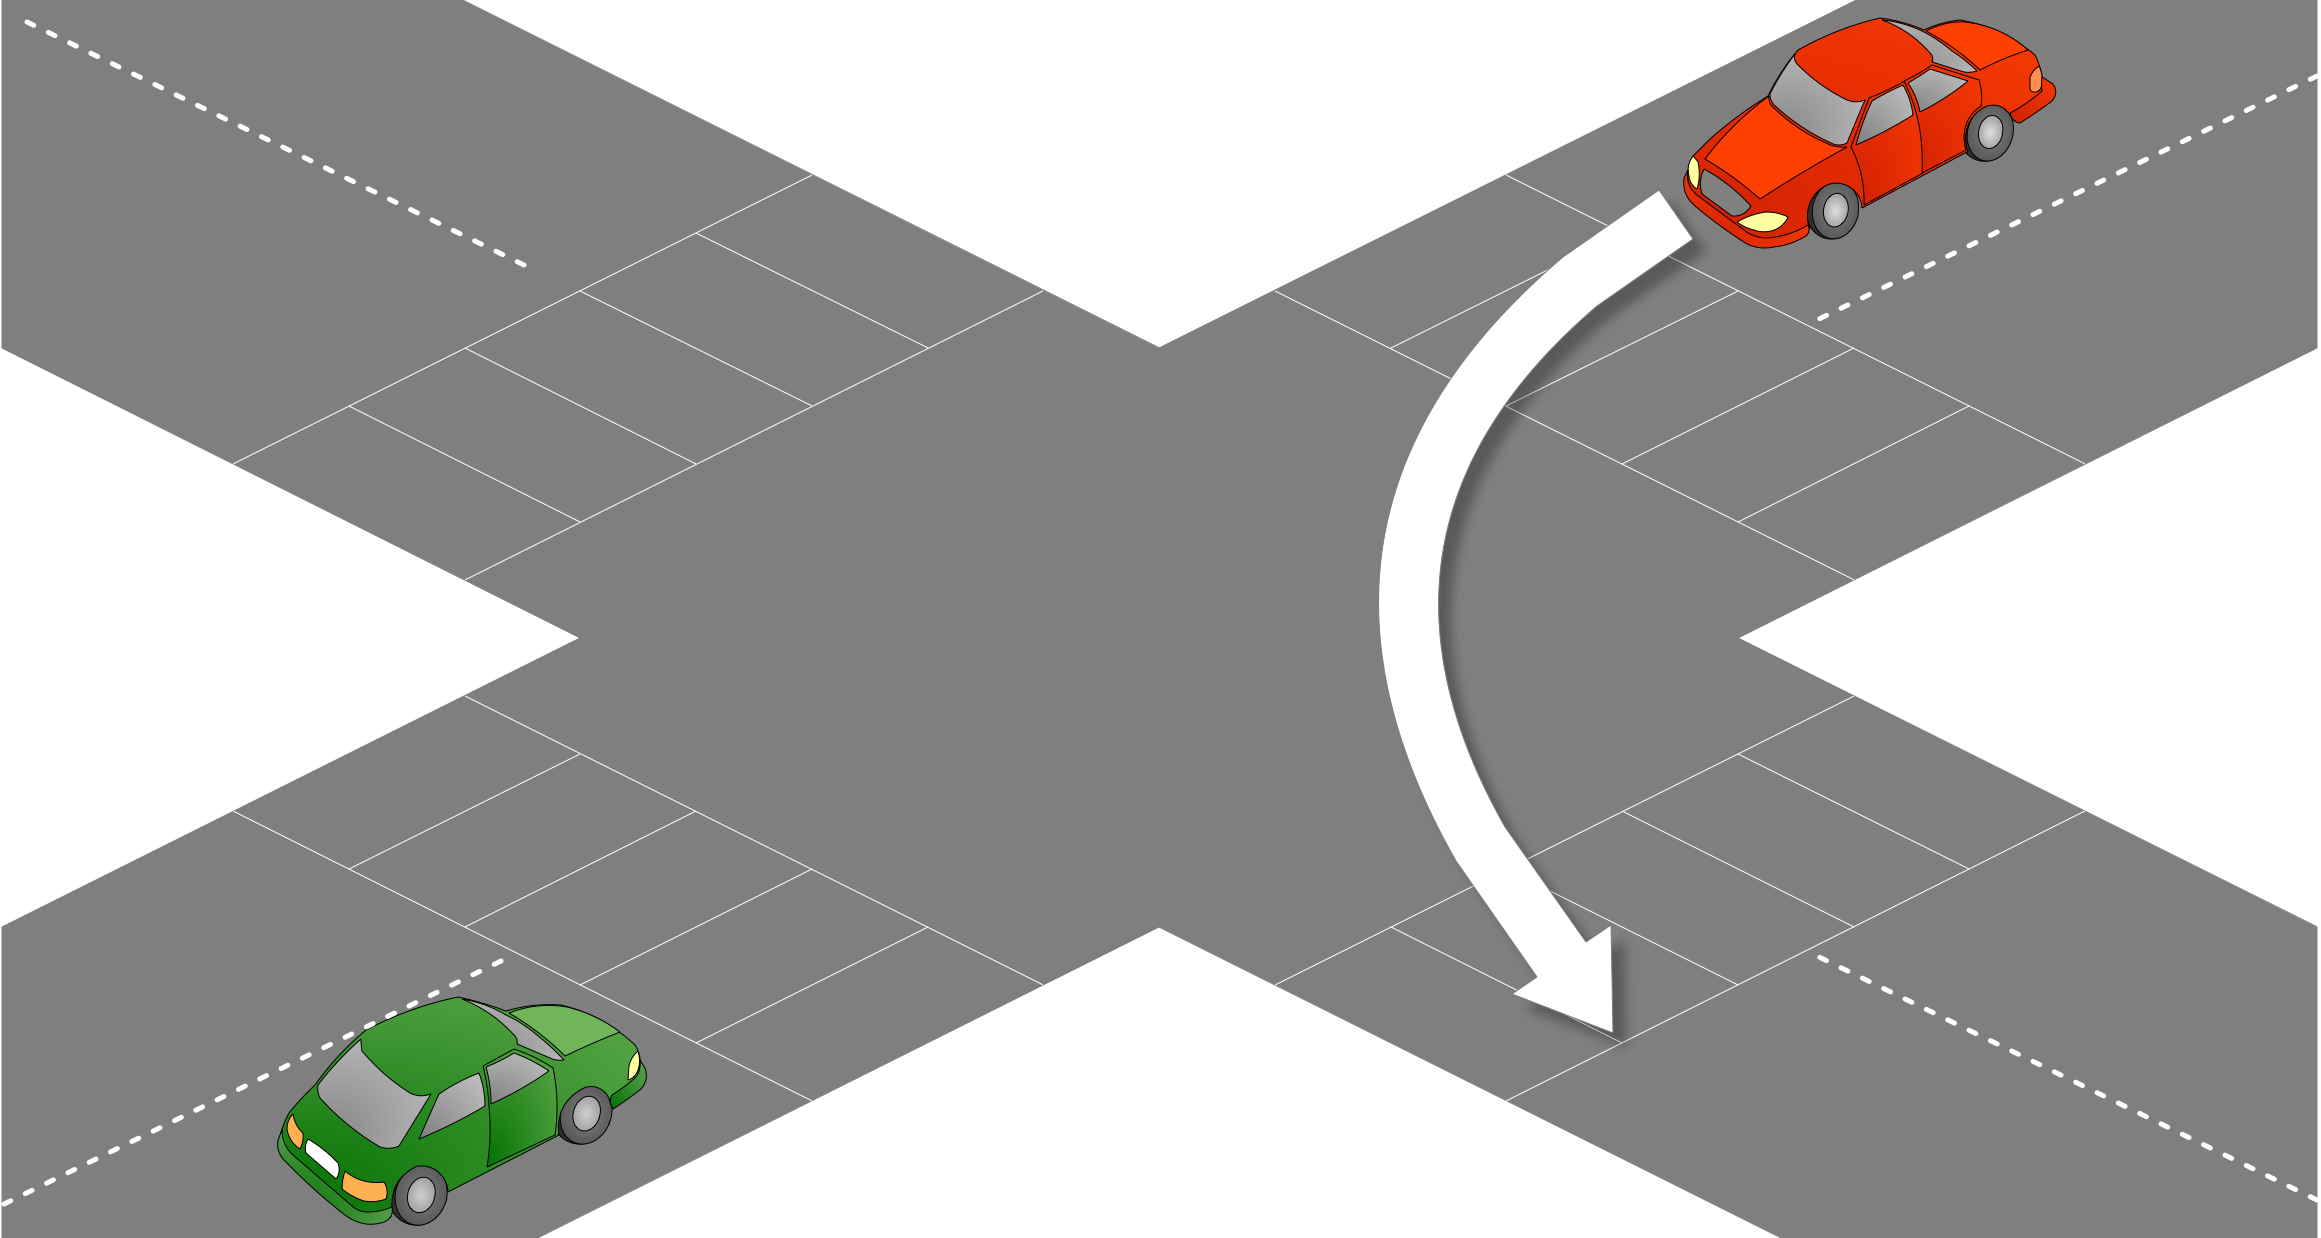
\includegraphics[width=0.45\textwidth]{text/figures/leftIntersect.png} \label{fig:introduction:semantics:d}}\\
    
    \subfloat[\tiny{Other vehicle entering intersection - straight across path.}]{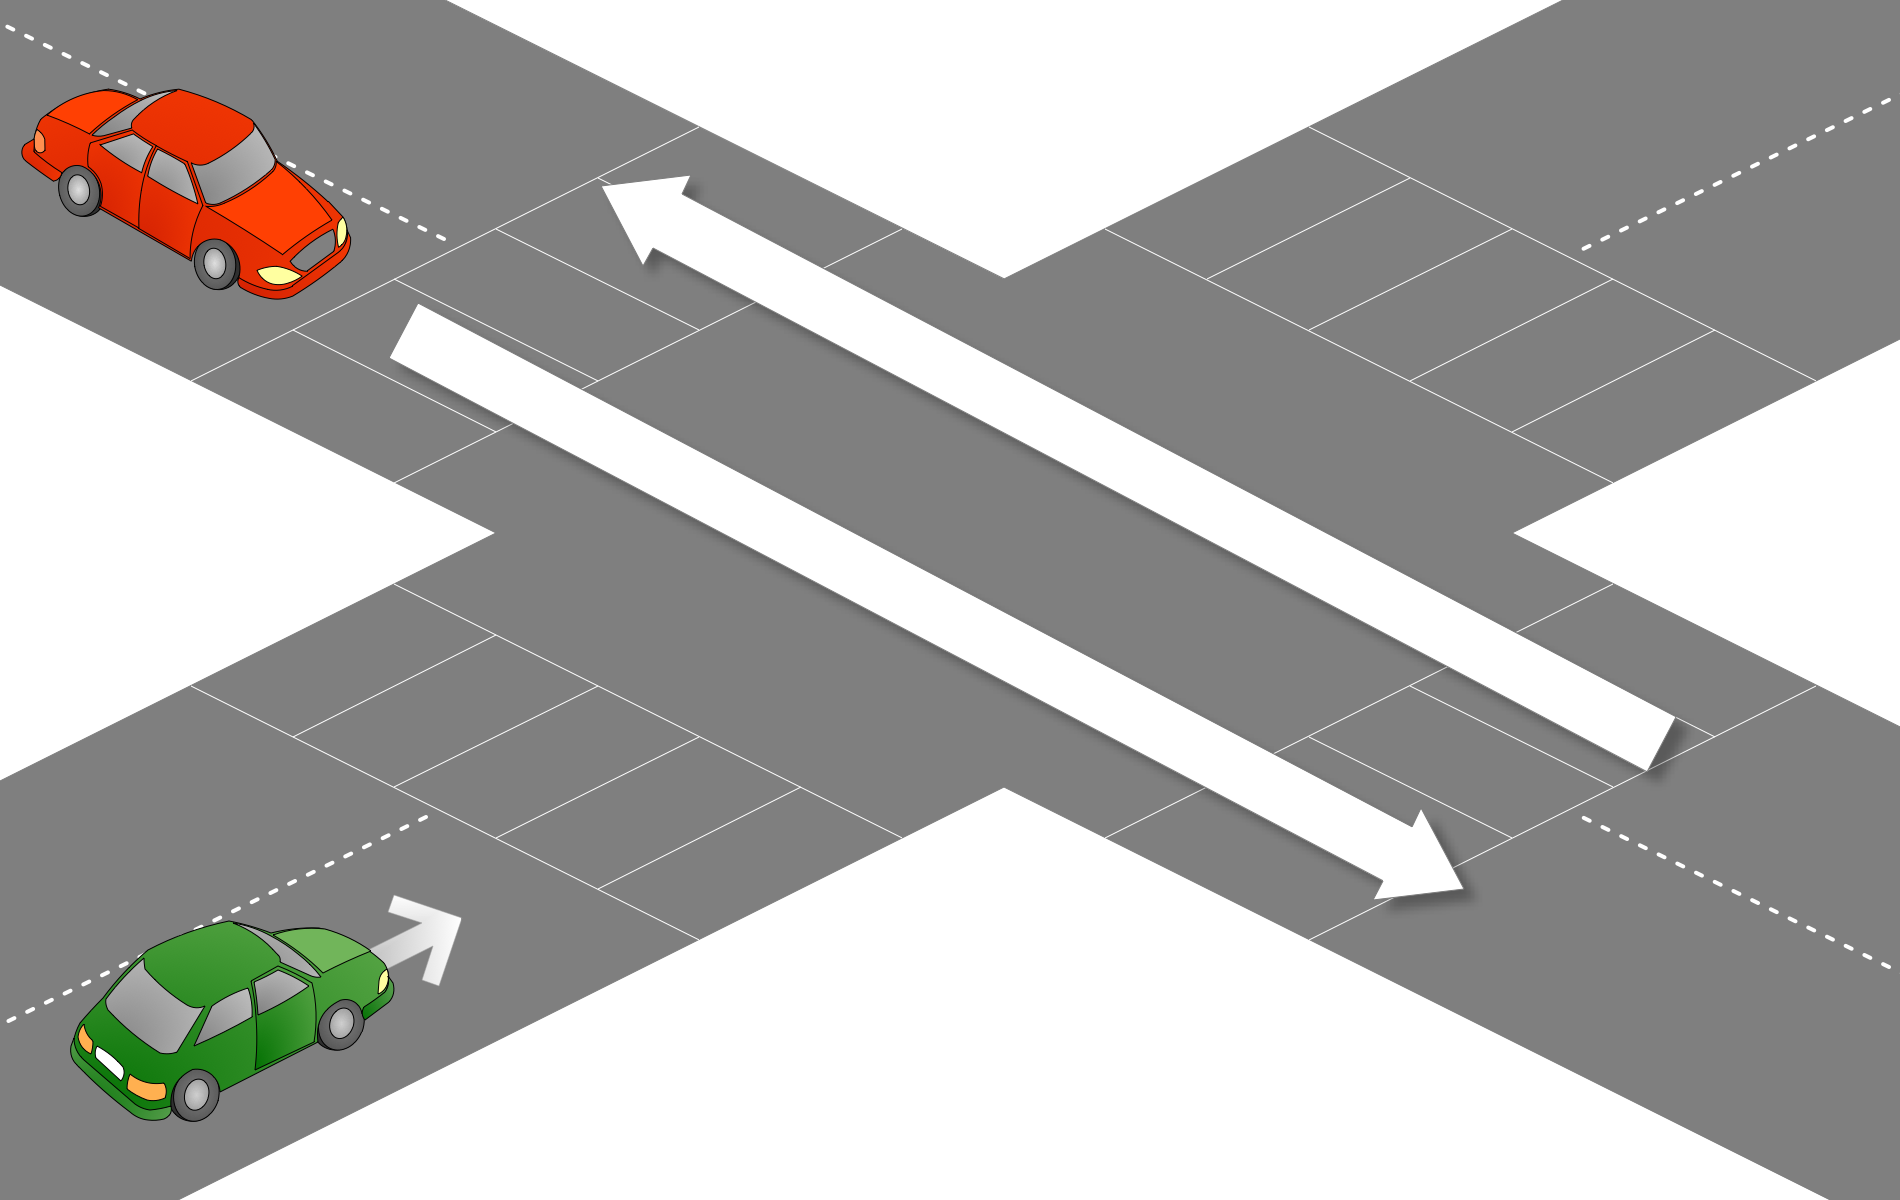
\includegraphics[width=0.45\textwidth]{text/figures/passingIntersect.png} \label{fig:introduction:semantics:e}} &
    \subfloat[\tiny{Other vehicle entering intersection - turning onto same direction.}]{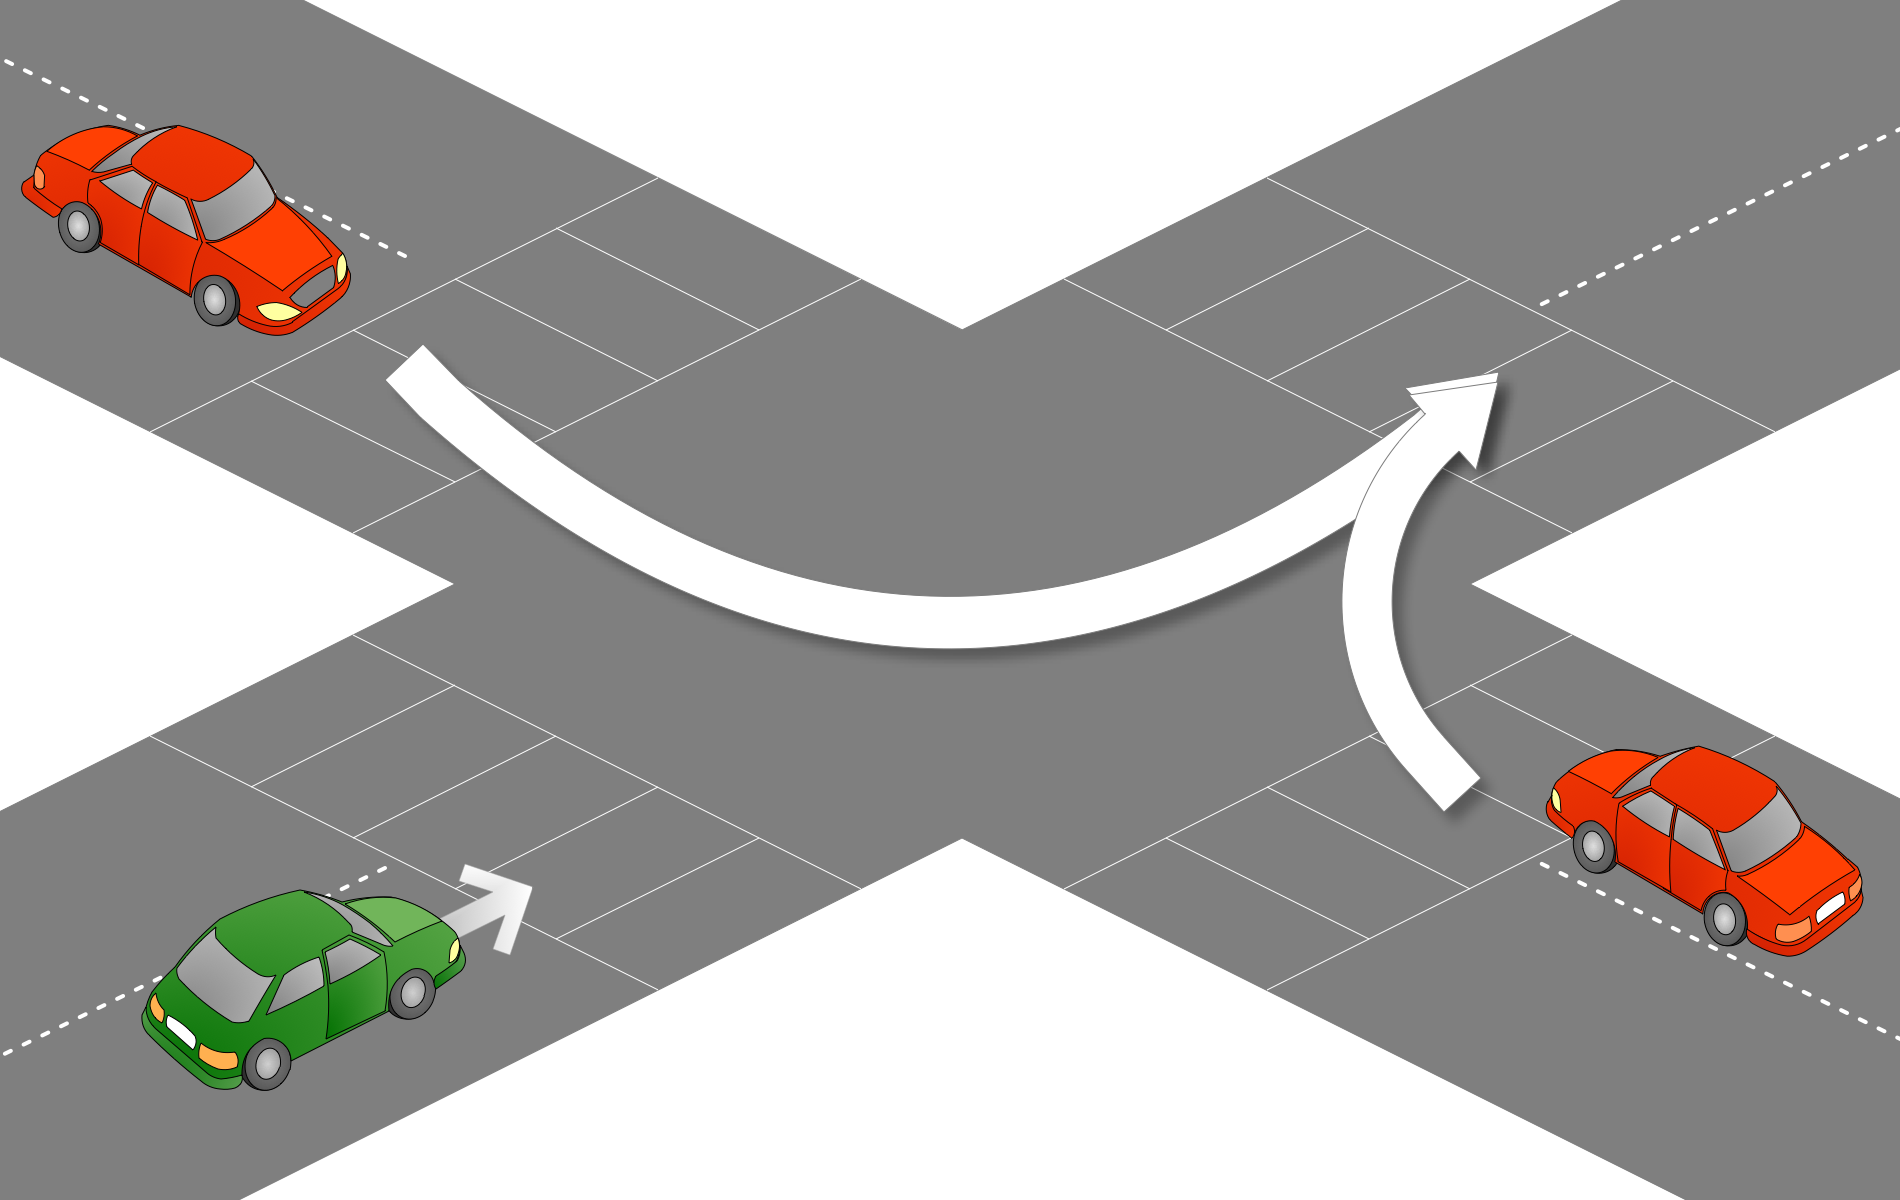
\includegraphics[width=0.45\textwidth]{text/figures/passingIntersectOntoSameDirection.png} \label{fig:introduction:semantics:f}}
  \end{tabular}
  \caption{\scriptsize{Automatically detectable critical events. Green car is ego vehicle moving towards intersection. Red cars are other vehicles \cite{philipsen2015NDS}.} 
}
\label{fig:introduction:semantics}
\end{figure}
Monocular systems usually have problems dealing with occlusions since they detect based on appearance, something which require a large amount of training data and many not still be able to deal with all of the many possible viewpoints and light conditions. \\
%\vspace*{-3mm}



Our contributions are:
\begin{itemize}
\item Using stereo-vision for automatic event detection in both day and nighttime, with focus on intersections (Figure \ref{fig:introduction:semantics:a}, \ref{fig:introduction:semantics:c}, \ref{fig:introduction:semantics:d}, \ref{fig:introduction:semantics:e}, \ref{fig:introduction:semantics:f}).
%\item Using stereo-vision to determine: Average number of vehicles in front of the ego vehicle. (Figure \ref{fig:introduction:semantics:a}).
\item Introducing a new event: Average distance to vehicles directly in front of the ego vehicle. (Figure \ref{fig:introduction:semantics:b}).
\end{itemize}

\vspace{2pt}